\documentclass{article}
\usepackage{tkz-euclide}
\usepackage{calc}
\begin{document}

% \begin{tikzpicture}[scale=0.25]
%   \tkzSetUpLine[line width=1pt]
%   \tkzDefPoint(0,0){A}
%   \tkzDefPoint(17.54,0){B}
%   \tkzDefTriangle[two angles = 84 and 49](A,B)
%   \tkzGetPoint{C}
%   \tkzDrawPolygon(A,B,C)
%   \tkzLabelPoints[above](C)
%   \tkzLabelPoints[below](A,B)
%   \tkzMarkAngle[size=3](B,A,C)
%   \tkzLabelAngle[pos=5](B,A,C){$84^{\circ}$}
%   \tkzMarkAngle[size=3](A,C,B)
%   \tkzLabelAngle[pos=5](A,C,B){$x^{\circ}$}
%   \tkzLabelSegment[below](A,B){$17.54$}
%   \tkzLabelSegment[right](B,C){$23.8$}
% \end{tikzpicture}
%
% Q12.
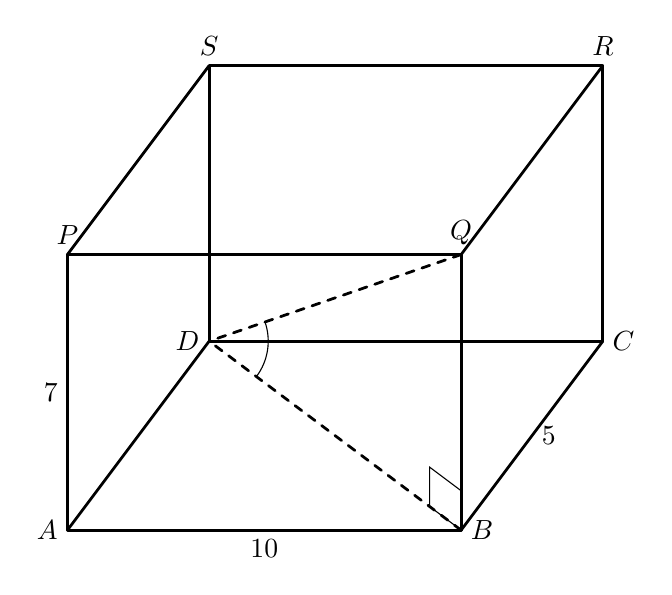
\begin{tikzpicture}[scale=.50]
  \tkzSetUpLine[line width=1pt]
  \tkzDefPoints{0/0/A,10/0/B,0/7/P,10/7/Q,6/0/a,2/0/b}
  \tkzDrawPolygon(A,B,Q,P)
  \tkzInterCC(A,a)(B,b) \tkzGetPoints{D}{}
  \tkzDefPointsBy[translation=from A to D](B,P,Q){C,S,R}
  \tkzDrawPolygon(D,S,R,C)
  \tkzDrawSegments[style=dashed](B,D Q,D)
  \tkzDrawSegments(A,D P,S Q,R B,C)
  \tkzLabelPoints[above](P,S,Q,R)
  \tkzLabelPoints[right](B,C)
  \tkzLabelPoints[left](A,D)
  \tkzMarkAngle[size=1.5](B,D,Q)
  \tkzMarkRightAngle[size=1](Q,B,D)
  \tkzLabelSegment[left](A,P){$7$}
  \tkzLabelSegment[below](A,B){$10$}
  \tkzLabelSegment[right](B,C){$5$}
\end{tikzpicture}

% % Q11.
% \begin{tikzpicture}[scale=.75]
%   \tkzSetUpLine[line width=1pt]
%   \tkzDefPoints{0/0/A,5/0/B,12/5/c,0/7/v}
%   \tkzDefParallelogram(A,B,c)
%   \tkzGetPoint{d}
%   \tkzInterLC(A,d)(A,B) \tkzGetPoints{}{D}
%   \tkzInterLC(B,c)(B,A)  \tkzGetPoints{C}{}
%   \tkzDrawPolygon(A,B,C,D)
%   \tkzLabelPoints[left](A,D)
%   \tkzLabelPoints[right](B,C)
%   \tkzDefMidPoint(A,C) \tkzGetPoint{X}
%   \tkzDrawPoint(X)
%   \tkzLabelPoints[below](X)
%   \tkzDefLine[perpendicular=through X,K=1](D,C)
%   \tkzGetPoint{n}
%   \tkzInterLC(X,n)(A,v) \tkzGetPoints{}{V}
%   \tkzLabelPoints[left](V)
%   \tkzDrawPolygon(A,V,B)
%   \tkzDrawSegments(A,C D,V C,V)
%   \tkzDrawSegments[style=dashed](X,V)
%   \tkzLabelSegment[pos=0.2, left](X,V){$7m$}
%   \tkzLabelSegment[below](A,B){$50m$}
%   \tkzLabelSegment[pos=0.75, left](A,D){$50m$}
% \end{tikzpicture}

% % Q10.
% \begin{tikzpicture}[scale=.60]
%   \tkzSetUpLine[line width=1pt]
%   \tkzDefPoints{0/0/A,6/0/B,12/6/c,0/9.95/v}
%   \tkzDefParallelogram(A,B,c)
%   \tkzGetPoint{d}
%   \tkzInterLC(A,d)(A,B) \tkzGetPoints{}{D}
%   \tkzInterLC(B,c)(B,A) \tkzGetPoints{C}{}
%   \tkzDrawPolygon(A,B,C,D)
%   \tkzLabelPoints[left](A,D)
%   \tkzLabelPoints[right](B,C)
%   \tkzDefMidPoint(A,B) \tkzGetPoint{M}
%   \tkzDrawPoint(M)
%   \tkzLabelPoints[below](M)
%   \tkzDefMidPoint(A,C) \tkzGetPoint{X}
%   \tkzDrawPoint(X)
%   \tkzLabelPoints[below](X)
%   \tkzDefLine[perpendicular=through X,K=1](D,C)
%   \tkzGetPoint{n}
%   \tkzInterLC(X,n)(A,v) \tkzGetPoints{}{V}
%   \tkzLabelPoints[left](V)
%   \tkzDrawPolygon(A,V,B)
%   \tkzDrawSegments(A,C D,V C,V)
%   \tkzDrawSegments[style=dashed](X,V)
%   \tkzLabelSegment[pos=0.2, left](X,V){$9m$}
%   \tkzLabelSegment[right](B,C){$6m$}
% \end{tikzpicture}

% Q8.
% \begin{tikzpicture}[scale=.60]
%   \tkzSetUpLine[line width=1pt]
%   \tkzDefPoints{0/0/C,6/0/B,0/10.77/D,0/6.77/d,-2/0/b}
%   \tkzDrawSegments(C,B C,D)
%   \tkzInterCC(D,d)(B,b) \tkzGetPoints{A}{}
%   \tkzDrawPolygon(A,B,C,D)
%   \tkzDrawSegments(C,A)
%   \tkzMarkAngle[size=1.7](A,C,D)
%   \tkzLabelAngle[pos=2.3](A,C,D){$\theta$}
%   \tkzLabelPoints(C,B)
%   \tkzLabelPoints[left](D)
%   \tkzLabelPoints[right](A)
%   \tkzLabelSegment[above](D,A){$4$}
%   \tkzLabelSegment[right](A,B){$8$}
%   \tkzLabelSegment[below](C,B){$6$}
%   \tkzLabelSegment[left](D,C){$10.77$}
% \end{tikzpicture}

% Q5.
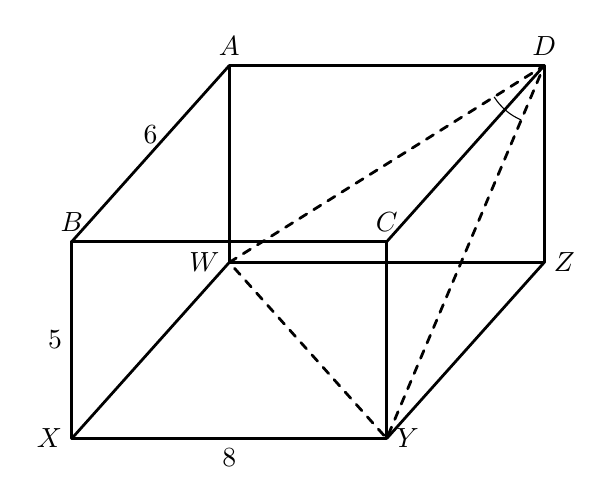
\begin{tikzpicture}[scale=.50]
  \tkzSetUpLine[line width=1pt]
  \tkzDefPoints{0/0/X,8/0/Y,0/5/B,8/5/C,6/0/x,2/0/y}
  \tkzDrawPolygon(X,Y,C,B)
  \tkzInterCC(X,x)(Y,y) \tkzGetPoints{W}{}
  \tkzDefPointsBy[translation=from X to W](Y,B,C){Z,A,D}
  \tkzDrawPolygon(A,D,Z,W)
  \tkzDrawPolygon[style=dashed](W,D,Y)
  \tkzDrawSegments(B,A C,D Y,Z X,W)
  \tkzLabelPoints[above](A,B,C,D)
  \tkzLabelPoints[left](W,X)
  \tkzLabelPoints[right](Y,Z)
  \tkzMarkAngle[size=1.5](W,D,Y)
  \tkzLabelSegment[left](B,X){$5$}
  \tkzLabelSegment(X,Y){$8$}
  \tkzLabelSegment[above](B,A){$6$}
\end{tikzpicture}

% % Q7
% \begin{tikzpicture}[scale=.75]
%   \tkzSetUpLine[line width=1pt]
%   \tkzDefPoints{2/4/P,4/8/Q,4/0/R}
%   \tkzDrawPolygon(P,Q,R)
%   \tkzLabelPoints[left](P,Q,R)
%   \tkzMarkAngle[size=1](P,Q,R)
%   \tkzLabelAngle[pos=1.5](P,Q,R){$\theta$}
% \end{tikzpicture}

% % Q9
% \begin{tikzpicture}[scale=.50]
%   \tkzSetUpLine[line width=1pt]
%   \tkzDefPoints{0/0/B,0/7.10/A,7.81/0/C}
%   \tkzDrawPolygon(B,A,C)
%   \tkzLabelPoints[left](A)
%   \tkzLabelPoints[below](B,C)
%   \tkzMarkAngle[size=1](C,B,A)
%   \tkzLabelAngle[pos=1.7](C,B,A){$95^{\circ}$}
%   \tkzMarkAngle[size=1](A,C,B)
%   \tkzLabelAngle[pos=1.7](A,C,B){$40^{\circ}$}
%   \tkzLabelSegment[right](A,C){$11$}
% \end{tikzpicture}

% \begin{tikzpicture}
%   \tkzSetUpLine[line width=1pt]
%   \tkzDefPoints{0/0/A,4/0/B,0/4/E,4/4/F}
%   \tkzDrawPolygon(A,B,F,E)
%   \tkzInterLC(A,F)(A,B) \tkzGetPoints{}{D}
%   \tkzDefPointsBy[translation=from A to D](E,F,B){H,G,C}
%   \tkzLabelPoints(A,B,C)
%   \tkzLabelPoints[left](D)
%   \tkzLabelPoints[above](H,G,E,F)
%   \tkzDrawSegments(E,H F,G B,C H,G C,G)
%   \tkzDrawSegments[color=gray, style=dashed](D,A D,C D,H B,H D,B)
%   \tkzMarkAngle[size=1](H,B,D)
%   \tkzLabelAngle[pos=1, left](H,B,D){$x^{\circ}$}
% \end{tikzpicture}

% \begin{tikzpicture}[>=latex]
%   \tkzDefPoints{0/0/A,3/0/B,3/1/A',1/2/C}
%   \tkzDefPointsBy[translation= from A to A'](B,C){}
%   \tkzDrawPolygon(A,B,C)
%   \tkzDrawPolygon(A',B',C')
%   \tkzDrawPoints(A,B,C)
%   \tkzDrawPoints(A',B',C')
%   \tkzLabelPoints(A,B,A',B')
%   \tkzLabelPoints[above](C,C')
%   \tkzDrawSegments[color = gray,->, style=dashed](A,A' B,B' C,C')
% \end{tikzpicture}

% \begin{tikzpicture}[scale=.75]
%   \tkzSetUpLine[line width=1pt]
%   \begin{scope}[rotate=-80]
%     \tkzDefPoints{0/6/A,10/0/B,10/6/C}
%     \tkzDefPointBy[projection = onto B--A](C)
%     \tkzGetPoint{H}
%     \tkzMarkRightAngle[size=.4, fill=teal!20](B,C,A)
%     \tkzMarkRightAngle[size=.4, fill=orange!20](B,H,C)
%     \tkzDrawPolygon(A,B,C)
%     \tkzDrawSegment(C,H)
%   \end{scope}
%   \tkzLabelSegment[below](C,B){$a$}
%   \tkzLabelSegment[right](A,C){$b$}
%   \tkzLabelSegment[left](A,B){$c$}
%   \tkzLabelSegment[color=red](C,H){$h$}
%   \tkzDrawPoints(A,B,C)
%   \tkzLabelPoints[above left](H)
%   \tkzLabelPoints(B,C)
%   \tkzLabelPoints[above](A)
% \end{tikzpicture}

% \begin{tikzpicture}[scale=0.30]
%   \tkzDefPoint(0,0){A}
%   \tkzDefPoint(9,0){C}
%   \tkzDefTriangle[two angles = 66 and 85](A,C)
%   \tkzGetPoint{B}
%   \tkzDrawPolygon(A,B,C)
%   \tkzLabelPoints[above](B)
%   \tkzLabelPoints[below](A,C)
%   \tkzMarkAngle[size=3](C,A,B)
%   \tkzLabelAngle[pos=5](C,A,B){$66^{\circ}$}
%   \tkzMarkAngle[size=3](A,B,C)
%   \tkzLabelAngle[pos=5](A,B,C){$29^{\circ}$}
%   \tkzLabelSegment[right](B,C){$x$}
%   \tkzLabelSegment[below](A,C){$9$}
% \end{tikzpicture}

% \begin{tikzpicture}[scale=0.75]
%   \tkzDefPoint(0,0){A}
%   \tkzDefPoint(8,0){B}
%   \tkzDefTriangle[two angles = 90 and 32](A,B)
%   \tkzGetPoint{C}
%   \tkzDrawPolygon(A,B,C)
%   \tkzDefTriangle[two angles = 71 and 18](A,B)
%   \tkzGetPoint{M}
%   \tkzGetPointCoord(M){m}
%   \tkzDefPoint(\mx,-\my){D}
%   \tkzDrawPolygon(A,D,B)
%   \tkzLabelPoints[above](C)
%   \tkzLabelPoints[below](B,D)
%   \tkzLabelPoints[left](A)
%   \tkzMarkAngle[size=1](A,C,B)
%   \tkzLabelAngle[pos=1.5](A,C,B){$58^{\circ}$}
%   \tkzMarkAngle[size=0.7](D,A,B)
%   \tkzLabelAngle[pos=1.2](D,A,B){$71^{\circ}$}
%   \tkzMarkRightAngle[size=1](C,A,B)
%   \tkzMarkRightAngle[size=0.7](B,D,A)
%   \tkzLabelSegment[above](A,B){$8$}
%   \tkzLabelSegment[below](D,B){$x$}
% \end{tikzpicture}

% \begin{tikzpicture}[scale=0.07]
%   \tkzDefPoint(0,0){C}
%   \tkzDefPoint(113.45906750894791,0){A}
%   \tkzDefPoint(0,53.6){D}
%   \tkzDrawPolygon(A,C,D)
%   \tkzLabelPoints(C)
%   \tkzLabelPoints[above](A)
%   \tkzLabelPoints[above](D)
%   \tkzDefTriangle[two angles = 90 and 3.993](A,D)
%   \tkzGetPoint{B}
%   \tkzLabelPoints[below](B)
%   \tkzDrawPolygon(A,D,B)
%   \tkzMarkRightAngle[size=7](D,C,A)
%   \tkzMarkRightAngle[size=3](D,A,B)
%   \tkzMarkAngle[size=13](D,A,C)
%   \tkzLabelAngle[pos=17](D,A,C){$x^{\circ}$}
%   \tkzLabelSegment[right](A,B){$6.98$}
%   \tkzLabelSegment[above](D,A){$100$}
%   \tkzLabelSegment[left](D,C){$53.6$}
% \end{tikzpicture}

% \begin{tikzpicture}[scale=0.50]
%   \tkzGrid
%   \tkzDefPoint(0,0){C}
%   \tkzDefPoint(3,0){A}
%   \tkzLabelPoints(A,C)
%   \tkzDefShiftPoint[A](0,5){Z}
%   \tkzDrawPoints(Z)
%   \tkzLabelPoints(Z)
% \end{tikzpicture}

% \begin{tikzpicture}[scale=0.40]
%   % \tkzInit[xmax=25, ymax=20]
%   % \tkzGrid
%   \tkzDefPoint(0,0){B}
%   \tkzDefPoint(23.8,0){C}
%   \tkzDefTriangle[two angles = 50 and 47](B,C)
%   \tkzGetPoint{A}
%   \tkzDrawPolygon(A,B,C)
%   \tkzLabelPoints[above](A)
%   \tkzLabelPoints(B,C)
%   \tkzMarkAngle(C,B,A)
%   \tkzLabelAngle[pos=2](C,B,A){$50^\circ$}
%   \tkzMarkAngle(B,A,C)
%   \tkzLabelAngle[pos=2](B,A,C){$83^\circ$}
%   \tkzLabelSegment[right,above](C,A){$b$}
%   \tkzLabelSegment[left,above](A,B){$c$}
%   \tkzLabelSegment[below](B,C){$a=23.8$}
% \end{tikzpicture}

% \begin{tikzpicture}
%   \tkzDefPoints{0/0/A,5/0/B}
%   \tkzDrawSegment(A,B)
%   \tkzDefPointBy[rotation=center A angle 60](B)
%   \tkzGetPoint{C}
%   \tkzDefPointBy[symmetry=center C](A)
%   \tkzGetPoint{D}
%   \tkzDrawSegment(A,tkzPointResult)
%   \tkzDrawLine(B,D)
%   \tkzDrawArc(A,B)(C)
%   \tkzDrawArc(B,C)(A)
%   \tkzDrawArc(C,D)(D)
%   \tkzMarkRightAngle(D,B,A)
%   \tkzDrawPoints(A,B)
%   \tkzLabelPoints(A,B)
%   \tkzLabelPoints[above](C)
%   \tkzLabelPoints[right](D)
% \end{tikzpicture}

% \begin{tikzpicture}[scale=0.40]
%   \tkzInit[xmax=25, ymax=20]
%   \tkzGrid
%   \tkzDefPoints{0/0/B,23.8/0/X}
%   \tkzDrawSegment(B,X)
%   \tkzLabelPoints(B)
%   \tkzDefPointBy[rotation=center B angle 50](X)
%   \tkzGetPoint{C}
%   \tkzLabelPoints[above](C)
%   \tkzDrawSegment(B,C)
%   % \tkzDefTriangle[euclid](B,C) \tkzGetPoint{A}
%   % \tkzDrawPolygon{A,B,C}
%   % \tkzLabelSegment[below](C,B){$12cm$}
%   % \tkzLabelPoints[above](A)
%   % \tkzDrawSegment(C,A)
%   % \tkzLabelSegment[left](C,A){$10cm$}
%   % \tkzDrawSegment(B,A)
%   % \tkzMarkAngle (B,C,A)
%   % \tkzLabelAngle[pos=1.8](B,C,A){$48^{\circ}$}
% \end{tikzpicture}

% \begin{tikzpicture}
%   \tkzDefPoint(0,0){C} \tkzDefPoint(4,0){D}
%   \tkzDefSquare(C,D)
%   \tkzGetPoints{e}{f} \tkzDefMidPoint(C,f)
%   \tkzGetPoint{m}
%   \tkzInterLC(C,f)(m,e) \tkzGetSecondPoint{n}
%   \tkzInterCC[with nodes](C,C,n)(D,C,n) \tkzGetFirstPoint{B} \tkzDrawSegment[brown,dashed](f,n) \pgfinterruptboundingbox % from tikz
%   \tkzDrawPolygon[brown,dashed](C,D,e,f)
%   \tkzDrawArc[brown,dashed](m,e)(n)
%   \tkzCompass[brown,dashed,delta=20](C,B)
%   \tkzCompass[brown,dashed,delta=20](D,B)
%   \endpgfinterruptboundingbox
%   \tkzDrawPolygon(B,...,D)
%   \tkzDrawPoints(B,C,D,e,f,m,n)
%   \tkzLabelPoints[above](B)
%   \tkzLabelPoints[left](f,m,n)
%   \tkzLabelPoints(C,D)
%   \tkzLabelPoints[right](e)
% \end{tikzpicture}

\end{document}
